\documentclass[12pt,a4paper]{report}
\usepackage[margin=1in]{geometry}
\usepackage{titlesec}
\usepackage{amsmath}
\usepackage{amssymb}
\usepackage[colorlinks=true,urlcolor=black,linkcolor=black]{hyperref}
\usepackage{graphicx}
\usepackage{textcomp}
\usepackage{mathptmx}
\usepackage{tabto,enumitem}
\usepackage{algorithm}
\usepackage{algpseudocode}
\usepackage{wrapfig}

\titleformat{\chapter}{\bf\huge}{\thechapter}{20pt}{\huge\vspace{-.5em}}
    

\begin{document}

\begin{figure}
    \centering
    \begin{center}
    
\includegraphics[width=1.0\linewidth]{Images/Concordia-logo.jpeg}    
    \end{center}
    \label{fig:Concordia University Logo.}
\end{figure}

\title{SOEN 6011 : Software Engineering Processes\\[2.0em] 

\text{Project Report} \\
\textbf{Function 4 :  $\Gamma(x)$ Gamma Function} \\[1.5em] Submitted To : Dr. Pankaj Kamthan}

\author{Dhruviben Jigeshkumar Modi (40166396) }
\date{August 05, 2022}


\maketitle

\pagenumbering{roman}
\setcounter{page}{0}

\chapter{Problem 1}
\pagenumbering{arabic}

\section{Introduction}

F4: $\Gamma \left( x \right)$ which is known as Gamma function, is a generalization of the factorial function to non-integer numbers. The gamma function is defined as the improper integral of another function. It is denoted by a capital letter gamma from the Greek alphabet. \\

Let define f be the Gamma Function from A to B,therefore A is the domain and B is the  co-domain of the Gamma Function. \\
\indent(A)Domain of function: $\{x \in R^+: x > 0\}$ includes all complex numbers and the positive integer(except zero and negative integers).

(B)Co-domain of function: $(0, \infty]$\\
\indent\indent\indent When n in A is a positive integer, then the gamma function is related to the factorial function  $\Gamma(n) = (n-1)!$ \\
\indent\indent\indent When n in A for complex numbers with a positive real part, then the ${\displaystyle \Gamma (n)=\int _{0}^{\infty }x^{n-1}e^{-x}\,dx.}$

\begin{figure}[h]
    \centering
    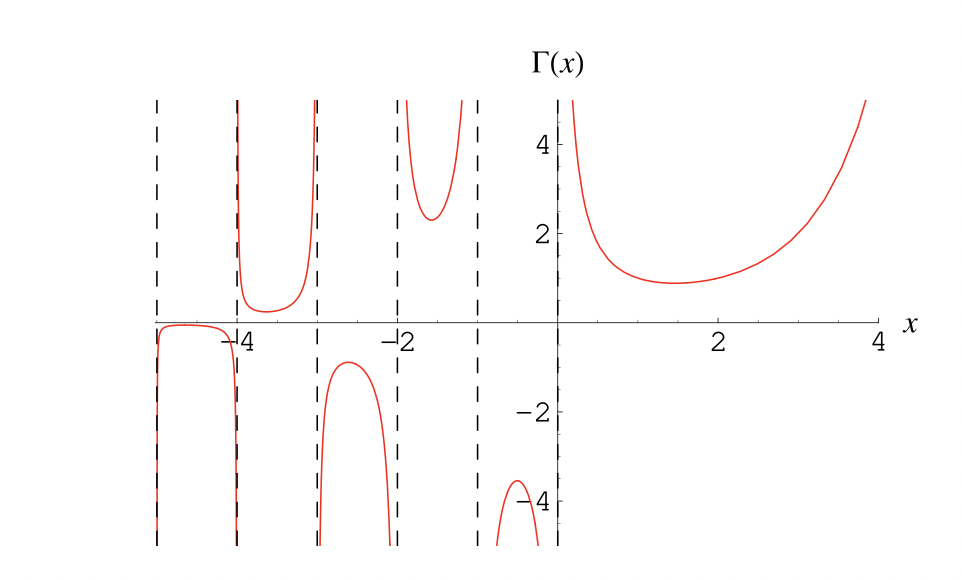
\includegraphics[width=0.4\linewidth]{Images/gammafun.png}
    \caption{Gamma Function}
    \label{fig:Gamma function}
\end{figure}

\section{Properties}
\indent\indent [1.] ${\displaystyle} n\to 0^+, {\displaystyle} \Gamma(n)\to+\infty$ \\

\indent [2.] Extreme property: a$\in\mathbf{R}$, $\lim_{n\to\infty} \frac{\Gamma(n+a)}{\Gamma(n)n^{a}} = 1, $ \\

\indent [3.] Density function: ${\displaystyle \Gamma \left(n+{\tfrac {1}{2}}\right)={\frac {(2n)!{\sqrt {\pi }}}{n!4^{n}}}}$ \\

\indent [4.] Recursive property: $\Gamma(n + 1)=n*\Gamma(n)$\\

\indent [5.] Euler's Reflection formula: $\Gamma(n)*\Gamma(1-n)=\frac{\pi}{\sin\pi n}$\\

\indent [6.] Legendre Duplication formula: $\Gamma(n)*\Gamma(n+\frac{1}{2})=2^{1-2n}*\sqrt{\pi}*\Gamma(2n)$\\

\indent [7.] For ${\lambda} > 0$, $ {\int _{0}^{\infty }x^{n-1}e^{-\lambda x}\,d} = \displaystyle \frac{\Gamma (n)}{\lambda^n}$\\

\section{Particular Values}
\indent\indent (1) $\Gamma(1) = 0! = 1$\\
\indent (2) $\Gamma(1/2) = \sqrt{\pi}$ \

\section{Context Use Model}

\begin{figure}[h]
    \centering
    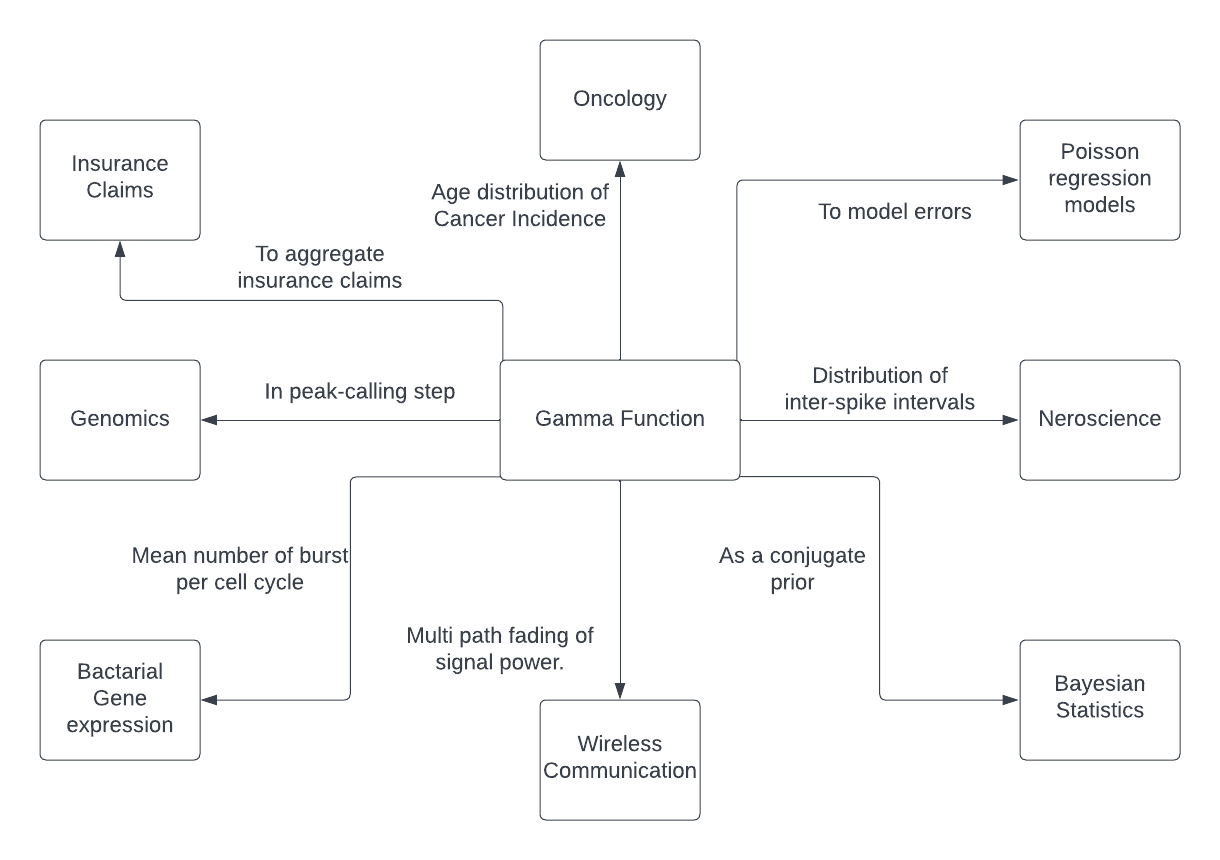
\includegraphics[width=0.9\linewidth]{Images/contextmodel.png}
    \caption{Context use model}
    \label{fig:context use model}
\end{figure}


\chapter{Problem 2}

\section{Explicit Assumption}
\begin{itemize}
     \item[1.]n is positive real number $n \in R^{+}$
     \item[2.]For n $\in Z^+$, it is easier to compute $\Gamma(n)$
\end{itemize}
\section{Requirements and corresponding properties}
\indent \textbf{F4 - $\Gamma \left( x \right)$} \\ \\
\indent (1) First Requirement : The Gamma Function $\Gamma(x)$ requires x as its variable input in order to proceed.

\begin{itemize}
    \item ID : FR1
    \item Version number: 1.0
    \item Priority: High
    \item Rationale: x
    \item Difficulty: Easy.
    \item Type: Functional requirement
\end{itemize}

(2) Second Requirement : If the user provides a legitimate input in domain of $R^+$, the Gamma function's output must be exact and correct.

\begin{itemize}
    \item ID : FR2
    \item Version number: 1.0
    \item Priority: High
    \item Rationale: $x > 0$, The fundamental goal of the calculating system is to provide an accurate answer quickly, hence this criteria is essential.
    \item Difficulty: Difficult, selection of correct algorithm.
    \item Type: Functional requirement
\end{itemize}

(3) Third Requirement : When the user entered the parameter x, Gamma calculator will check the value of a parameter. If the entered value is zero or negative it displays the error message. If the parameter is in form of String then exception is thrown with an error message.

\begin{itemize}
    \item ID : FR3
    \item Version number: 1.0
    \item Priority: High
    \item Rationale: For the gamma function, 0 and all the negative integers are not defined. For example ${\displaystyle \Gamma (0)=\int _{0}^{\infty }x^{-1}e^{-x}\,dx}$. It is not integrable. For small value of x, it appears to decay slowly, but for large values, it decays quite quickly. Non-Integral form is: \\\\
     $\lim_{a \to 0}\int _{a}^{1}x^{-1}e^{-x}dx \geq \frac{1}{e}\lim_{a \to 0}\int _{a}^{1} \frac{dx}{x}=\lim_{a \to 0}-log_a=\infty$ \\\\
    Thus $\Gamma \left( 0 \right)$ is undefined, and hence it is also undefined for all the negative integers.
    \item Difficulty: Easy
    \item Type: Functional requirement
\end{itemize}

(4) Fourth Requirement : To avoid a stack overflow, the gamma function can be calculated if the inputs are positive integers using the tail recursion function.

\begin{itemize}
    \item ID : FR4
    \item Version number: 1.0
    \item Priority: High
    \item Rationale: \{ $\forall n \in R^+$ $\mid\;$  $\Gamma(n)$ = $(n-1)! $ \}
    \item Difficulty: Moderate
    \item Type: Functional Requirements
\end{itemize}

(5) Fifth Requirement : The output of the gamma function can be computed for the fractional value of the input parameter using Stirling's approximation for performing definite integration.

\begin{itemize}
    \item ID : FR5
    \item Version number: 1.0
    \item Priority: High
    \item Rationale: \{ $\forall n \in R^{+}$ $\mid\;$y $\Gamma n = \sqrt{2 \cdot \pi \cdot n}\cdot (\frac{n}{e})^{n}$ \}
    \item Difficulty: Difficult
    \item Type: Functional Requirements
\end{itemize}

(6) Sixth Requirement : The system must be maintainable and managable to achieve usability.

\begin{itemize}
    \item ID : NFR1
    \item Version number: 1.0
    \item Priority: High
    \item Rationale: To make a system well-organized it is essential that each modules must be implemented separately, otherwise it is difficult to manage such complex system.
    \item Difficulty: Moderate
    \item Type: Non-Functional Requirement
\end{itemize}

(7) Seventh Requirement : The system portability.

\begin{itemize}
    \item ID : NFR2
    \item Version number: 1.0
    \item Priority: High
    \item Rationale: Java's architectural neutral features give the system the flexibility to function on many system architectures.
    \item Difficulty: Moderate
    \item Type: Non-Functional Requirement
\end{itemize}

(8) Eighth Requirement : The system Usability.

\begin{itemize}
    \item ID : NFR3
    \item Version number: 1.0
    \item Priority: High
    \item Rationale: Any user should be able to easily comprehend the system. For a novice user, error messages must be helpful.
    \item Difficulty: Easy
    \item Type: Non-Functional Requirement
\end{itemize}


\chapter{Problem 3}
\section{Gamma function with Lanczos}

\begin{algorithm}
\caption{Lanczos approximation for Gamma Function}

\textbf{Require:}  value: $x > 0$ \Comment{$x \in Z^{+}$} \\
\textbf{Ensure:} g is a constant that chosen randomly with the condition that  $ Re(z) > \frac{1}{2}$.

\begin{algorithmic}[1]

\Procedure {lanczosGamma}{x}
    \If x $< \frac{1}{2}$ then
    \State  $\Gamma (x)={\pi  \over \sin \pi x \Gamma (1-x)}$ \Comment{Reflection formula}
    \EndIf
    \State g $\leftarrow$  a small random integer
    \State P $\leftarrow$ a convergence of nine to ten terms \Comment{double floating-point precision.}
    
    
    \For {$i \leftarrow 1, P.length $}
    \State $P_{g}(x)=P_{0}+{\frac  {P_{i}}{x+i}}$
    \EndFor
    \State ${\displaystyle \Gamma (x+1)={\sqrt {2\pi }}{\left(x+g+{\tfrac {1}{2}}\right)}^{x+{\frac {1}{2}}}e^{-\left(x+g+{\frac {1}{2}}\right)}P_{g}(x)}$
    
    \State \textbf{return} $\Gamma (x)$
    \EndProcedure
\Statex

\State $result \leftarrow \Gamma (x)$ 

\end{algorithmic}
\end{algorithm}

Lanczos approximation is a method for computing the gamma function numerically, It is a practical alternative to the Stirling's approximation for calculating the gamma function with fixed precision.. The Lanczos approximation extends the factorial technique, which will be used to calculate input smaller than $0.5$, by using the reflection formula. It will apply a different formula for any other values. In order to compute the gamma function with standard single or double floating-point precision and select a fixed constant g, 9 to 10 terms of the series in an aggregate are required. These terms will all be used to determine the coefficients then incorporate it into the given formula ${\displaystyle \Gamma (x+1)={\sqrt {2\pi }}{\left(x+g+{\tfrac {1}{2}}\right)}^{x+{\frac {1}{2}}}e^{-\left(x+g+{\frac {1}{2}}\right)}P_{g}(x)}$.

\section{Gamma function with Stirling}

Stirling's estimate gives an approximate value for the factorial function n! or the gamma function $\Gamma(n)$ when $n>1$. For all positive integers, ${\displaystyle n!=\Gamma (n+1)}$ is applied. The approximation can most simply be derived for n an integer by approximating the sum over the terms of the factorial with an integral, so that ${\displaystyle \ln n! = n \ln(n) - n + \Theta \ln(n)}$. However  the gamma function, unlike the factorial, is more broadly defined for all complex numbers other than non-positive integers; nevertheless, Stirling's formula may still be applied. If $Re(x) > 0$ then, specifying the constant in $\mathcal{O}(\ln(n))$ error term gives $\frac{1}{2}\ln(2\pi n)$, yielding the more precise formula $n! \sim \sqrt {2\pi n} (\frac{n}{e})^n$. Stirling's approximation can be extended to the double inequality as follow $\sqrt {2\pi n} (\frac{n}{e})^n  e^\frac{1}{12n + 1} < n! < \sqrt {2\pi n} (\frac{n}{e})^n  e^\frac{1}{12n}$ 

\begin{algorithm}

\caption{Stirling's approximation for Gamma function}

\textbf{Require:}  value: $x > 0$ \Comment{$x \in Z^{+}$}\\
\textbf{Ensure:} x is large in absolute value
\begin{algorithmic}[1]

\Procedure {stirlingGamma}{x}
    \State \indent $\Gamma (x) = \Call{squareroot}{n}$  \Comment{formula is an asymptotic expansion}
    
    \State \textbf{return} $\Gamma (x)$
    
    \Procedure{squareRoot}{n}
    \State error $\leftarrow$ 0.00001
    \State errorPrecision $\leftarrow$ 1
    \State temp $\leftarrow$ n
    \While {$errorPrecision > error$}
        \State $n \leftarrow \frac{{n}+ \frac{temp}{n}}{2}$
        \State $errorPrecision \leftarrow n - \frac{temp}{n}$
    \EndWhile
    \State \textbf{return} $n$
    \EndProcedure
    
    \Procedure{Power}{$base, exponent$}
    \State Convert the exponent into String
    \State $exponentArray \leftarrow Split\; the\; exponent\; into\; integer\; and\; fractional\; part $
    \If {$exponentArray[1] > 0$} 
     \State \qquad \textbf{return} $\Call{fractionPower}{base, exponent}$ \Comment{it returns fractionPower}
     \EndIf
     \If {$ exponent < 0$} 
     \State \qquad $base \leftarrow 1/base$
     \State \qquad $exponent \leftarrow exponent * (-1)$
     \State \textbf{return} \Call{power}{base, exponent} \Comment{it returns the power}
     \EndIf
     \State else if $exponent \leftarrow 0$ then
     \State \qquad \textbf{return} 1 \Comment{it returns 1}
     \State else if  $exponent \mod  2 \leftarrow 0$ then 
     \State \qquad $base \leftarrow base * base $
     \State \qquad $exponent \leftarrow exponent/2 $
     \State \textbf{return} \Call{exponent}{base , exponent} \Comment{it returns power}
     \State else
     \State \qquad $exponent \leftarrow (exponent-1)/2$
     \State \textbf{return}\; $base$ * \Call{power}{base * base , exponent} \Comment{it returns the power}
    \EndProcedure

\EndProcedure
\end{algorithmic}
\end{algorithm}

\begin{algorithm}
\begin{algorithmic}[1]
    \Procedure{stirlingGamma}{x}
    \Procedure{fractionPower}{$base, exponent$}
    \If {$exponent \leftarrow 0$}
    \State \qquad \textbf{return} 1.0  \Comment{it returns the value 1}
    \EndIf
    \If {$base < 0$} 
    \State \qquad $ln \leftarrow \Call{logarithm}{base * (-1)}$
    \EndIf
    \State else
    \State \qquad $ln \leftarrow \Call{logarithm}{base}$
    \If {$base \leftarrow 0$ and $exponent > 0$} 
    \State \qquad \textbf{return} answer \Comment{it returns the answer}
    \EndIf
    \For{$i \leftarrow 1, 125$}
    \State \qquad $u \leftarrow \Call{power}{exponent*ln , i}$
    \State \qquad $l \leftarrow \Call{factorial}{i}$
    \State \qquad answer = answer + (u/l)
    \EndFor 
    \If {$base < 0\;  $and$\;  exponent\;$ mod\; 2$ \neq  0$} 
    \State \qquad \textbf{return} $answer * (-1)$ \Comment{it returns the answer * (-1)}
    \EndIf
    \State else
    \State \qquad \textbf{return} answer; \Comment{it returns the answer}
    \EndProcedure
    
    \Procedure{logarithm}{n}
    \State $base \leftarrow (n - 1) / (n + 1)$
    \For{$i \leftarrow 1, 125$} 
    \State \qquad  $e \leftarrow {2*i-1}$
    \State \qquad $r \leftarrow {r+(1/e) * \Call{power}{base, exponent}}$
    \EndFor
    \State \textbf{return} 2 * $r$ \Comment{it returns a}
    \EndProcedure
    
    \Procedure{factorial}{$n$}
    \State \qquad \textbf{return}   \Call{factorialtailRecursion}{n,1} \Comment{it returns recursivefactorial function}
    \EndProcedure
    
    \Procedure{factorialtailRecusrion}{$n, a$}
    \If {$n \leftarrow 0$} 
    \State \qquad \textbf{return} a;\Comment{it returns a}
    \EndIf
    \State \textbf{return} \Call{factorialTailRecursive}{n-1 , n*a}\Comment{it returns factorialTailRecursive }
    \EndProcedure
    \EndProcedure
\Statex

\State $result \leftarrow \Gamma (x)$
\end{algorithmic}
\end{algorithm}


\newpage
\section{Advantages And Disadvantages}
\subsection{ The Lanczos approximation method}
\begin{itemize}
    \item{Performance : Evidently, the Lanczos approximation method increases efficiency compared to the original gamma function defined simply as ${\displaystyle \Gamma (x)=\int _{0}^{\infty }t^{x-1}e^{-t}\,dt}$ which need the integral calculating.}
    
    \item{Area of Application: Compared to the regular factorial function, which can only handle positive integers, the Lanczos approximation approach for the gamma function provides a wider range of applications. The method can be extended over the complete complex plane without the negative integer using the reflection formula, but it is only valid for arguments in the right complex half-plane when using the formula deduction.}
    
    \item{Accurateness : The outcome deviates slightly since the Lanczos approach is still only an approximation.}
    
    \item{Disadvantages : It can be challenging to calculate the Lanczos coefficients, and how well the calculations turn out relies on the two arbitrary parameters, g and n. Another disadvantage is that for fixed real parts of the free parameter, utilising complex coefficients increases calculation time while decreasing accuracy of the Lanczos approximation.}
\end{itemize} 

\subsection{ The Stirling's approximation method}
\begin{itemize}
    \item{Performance : Since it takes time to resolve convergent improper integration, the Stirling's approximation method is more efficient than the original gamma function.}
    
    \item{Area of Application: For any complex numbers other than non-positive integers, the Stirling's approximation for gamma function is more generally defined than the factorial, but Stirling's approximation can still be used.}
    
    \item{Accurateness : The benefit of the Stirling approximation approach is that even when the value of the parameter x is relatively small, the result is still quite accurate and results are almost identical when the value of the parameter x is large.}

    \item{Disadvantage : The drawback of this approach cannot comprehend real values that are less than or equal to $0$.}
\end{itemize}

\subsection{Conclusion}
The Stirling's approximation method is quite straightforward when compared to other gamma function implementation techniques.

\newpage
\section{MindMap}

\begin{figure}[h]
    \centering
    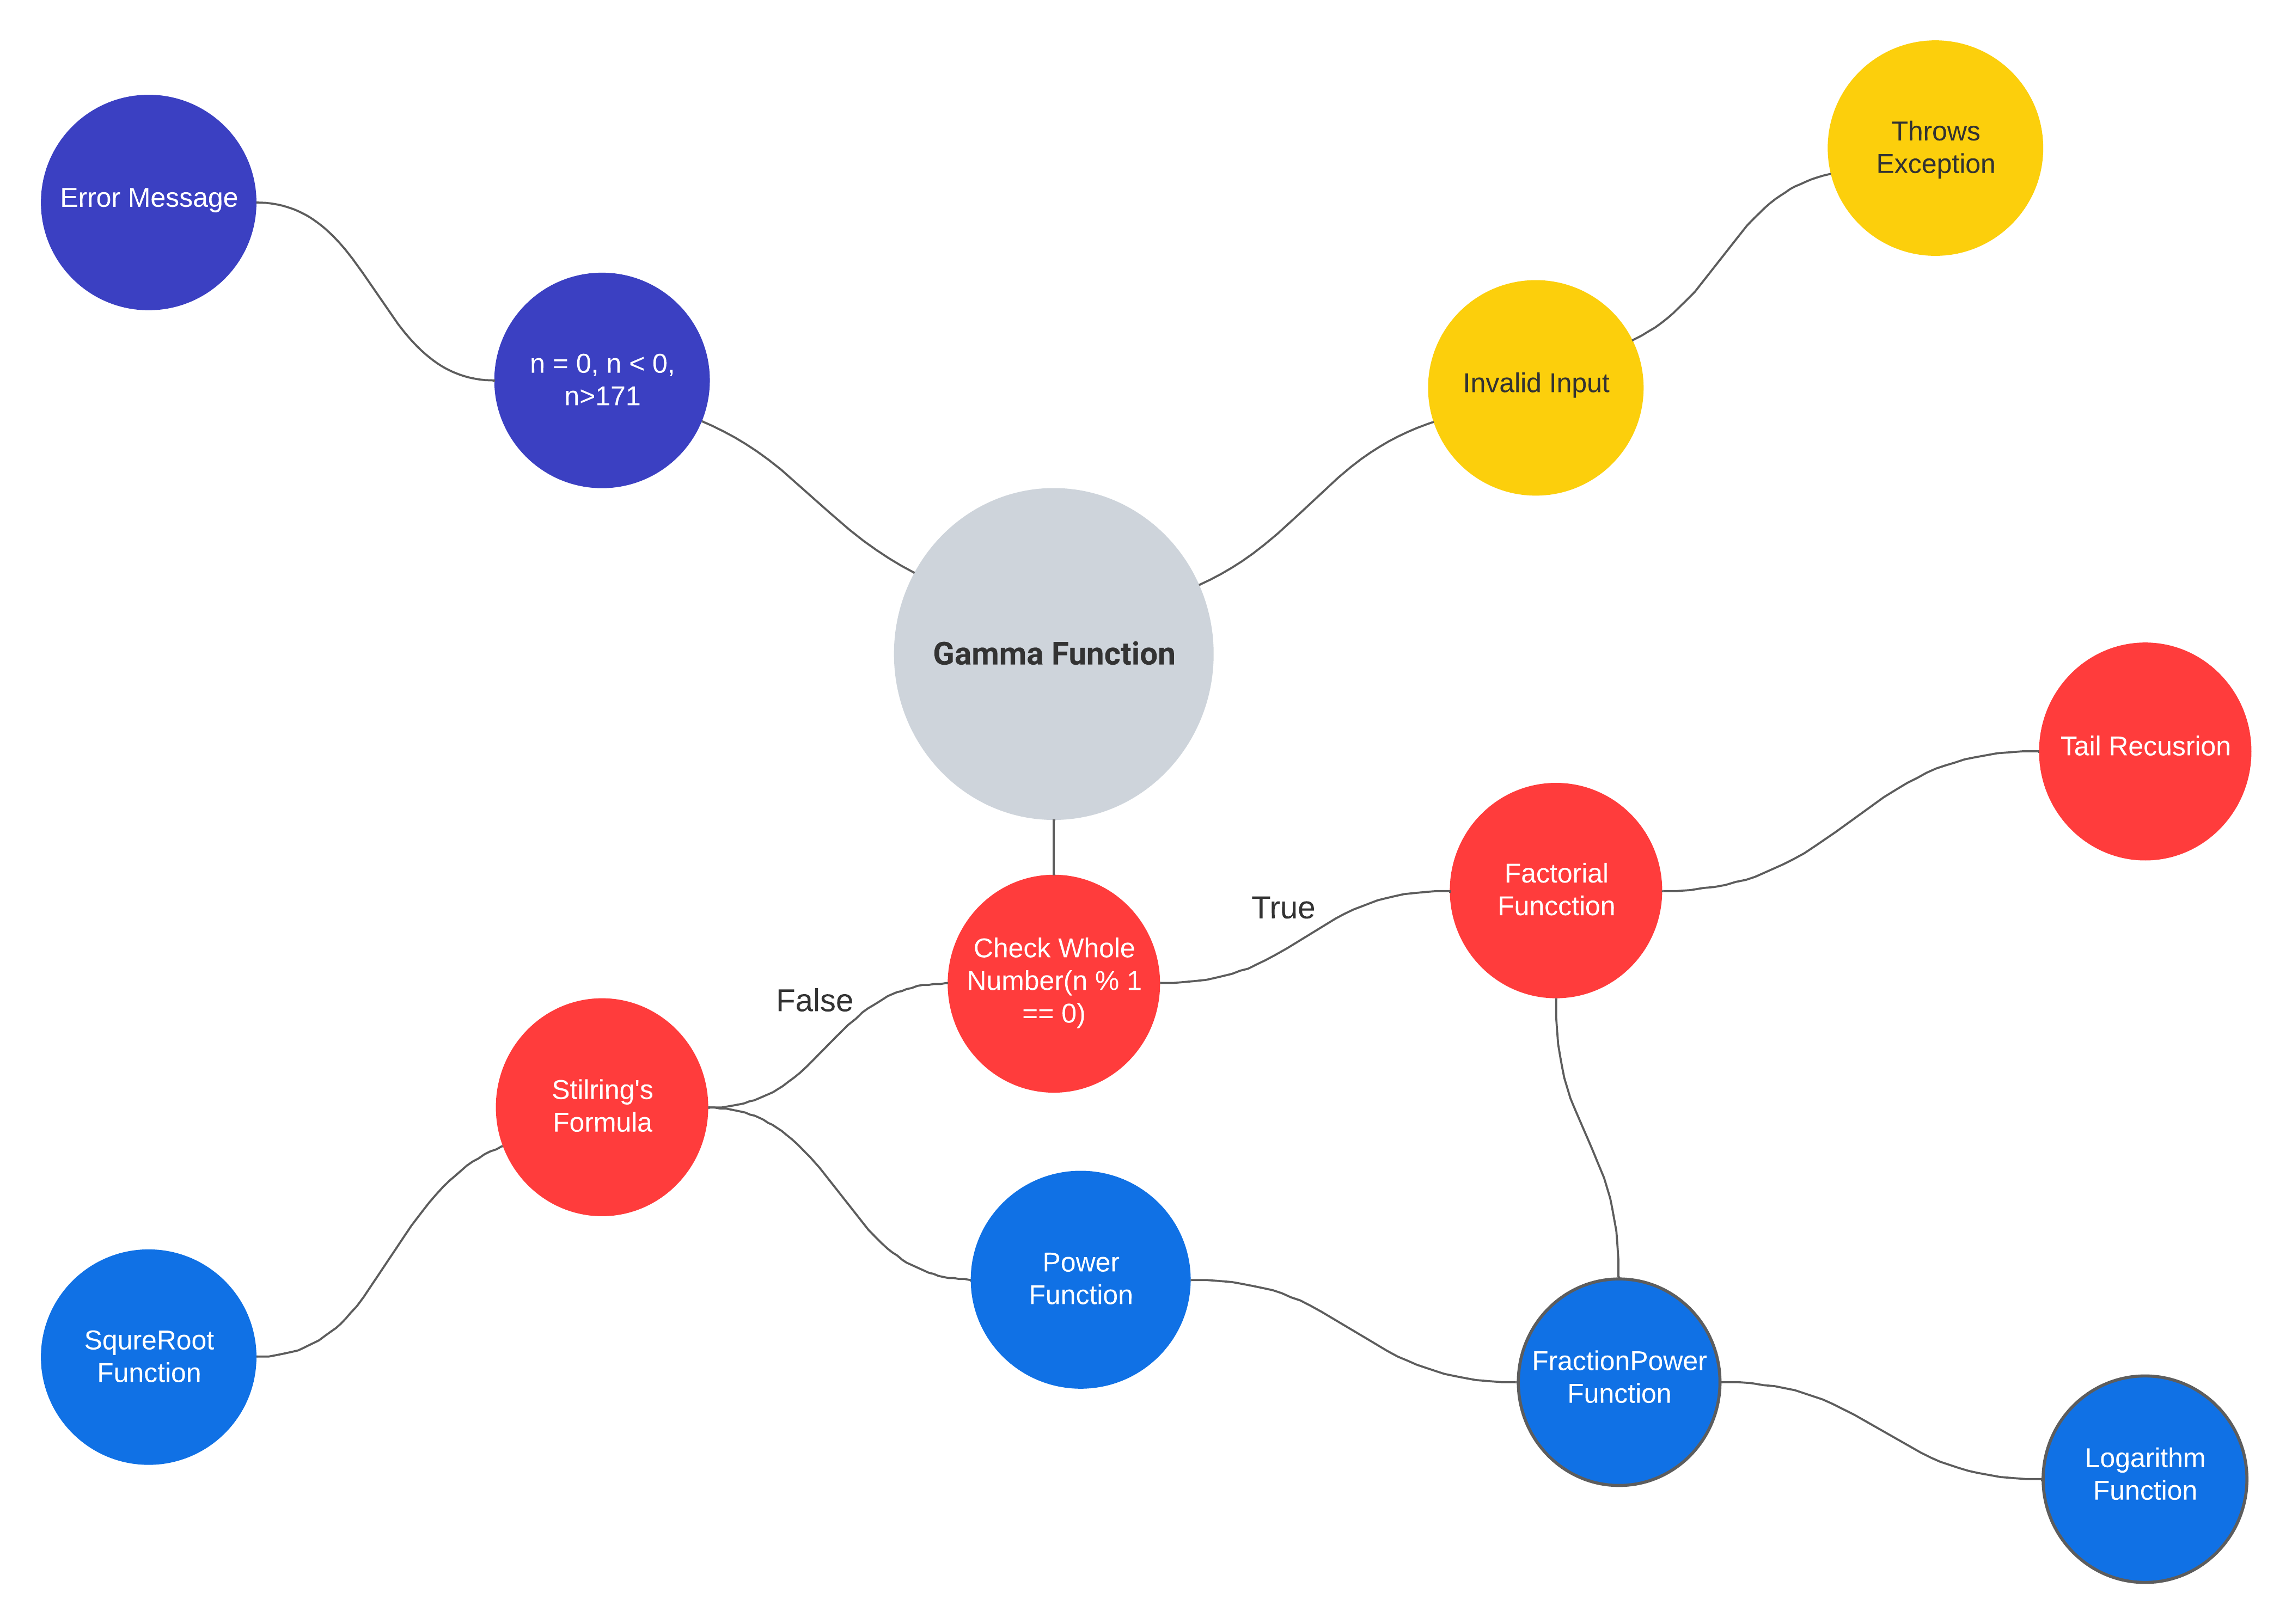
\includegraphics[width=1.0\linewidth]{Images/Mind map.png}
    \caption{MindMap to implement Gamma Function.}
    \label{fig:Exp_Data}
\end{figure}

\chapter{Problem 4}

\section{Error Handling and Messaging}
\indent\indent Maintaining the application's regular flow is the major benefit of exception handling. Exception is an unwanted or unexpected event, which occurs during the execution of a program\\

In Gamma Function calculator, if user enters any invalid input ($n = 0, n < 0, n > 171$), then the program will notify user with an error message containing "Infinity" as Gamma value of such numbers are positive infinity\\

Additionally, when a user accidentally enters a String, then in such case program throws an InputmisMatchException with a message that "Please enter correct input". In Gamma Function, exceptions are handled using try..catch method.\\

\section{Quality Attributes}
\begin{itemize}
    \item{Usability : To calculate the corresponding value of $\Gamma \left( n \right)$, the user only needs to enter the value of $n$, if the input is correct then the system returns the calculated value otherwise for the invalid input, the system also returns the exception that the input is not valid, which can help the user to easily perform the gamma function.}
    
    \item{Robustness : System can take positive real numbers, if the input is not valid then the system simply throws an exception and prints the error handling message containing "Invalid input", but the system will not crash. }
    
    \item{Efficient : The system is effective, which is made possible by a straightforward and uncomplicated method; As a result, the user will receive a prompt response within a second of entering correct input, whereas the system prints "Infinity" promptly when user enters $0$, less than $0$ and greater than $171$ as input. }
    
    \item{Maintainability : The separation of the function modules makes the system maintainable. The project's code follows standard programming practises, and each function and variable has a name that makes it clear what it does. Javadoc is written for each function hence the workload for maintenance is minimal.}
    
    \item{Correctness : The system's main requirement is correctness and precision. By using Stirling's formula for valid input, the application process will provide a reasonably accurate output.}
\end{itemize}

\newpage

\section{Debugger}
Finding and resolving errors in a program's source code is the process of debugging. Debugging tools are offered by contemporary IDEs like Eclipse, making it simpler for developers to interactively go through their code and analyse it to find and fix any flaws. To assist a developer in debugging successfully and efficiently, the Eclipse Java IDE offers a variety of debugging tools and perspectives grouped in the Debug Perspective.
\subsection{Advantages}
\begin{itemize}
    
    \item{It is efficient, does not require coding knowledge, and provides the greatest context for identifying issues.}
    
    \item{Error happens in a specific function, but code does not use that function until after the programme has been running for a while. Breakpoints specify where to "pause" a program's execution for the debugger. This makes it possible for you to access the desired area of the software fast.}
    
    \item{One of a debugger's most potent capabilities is single-stepping, which enables a reverse engineer to carry out a single instruction at a time before handing back control to the debugger.}
\end{itemize}

\subsection{Disadvantages}
\begin{itemize}
    \item{It requires human engagement, has a fair learning curve, is not always accessible, and cannot persist output.}
    
    \item{Another drawback of debugger is that the programmer cannot select which method to enter when there are several method calls because it lacks the wise step into function.}
\end{itemize}

\begin{figure}[h]
    \centering
    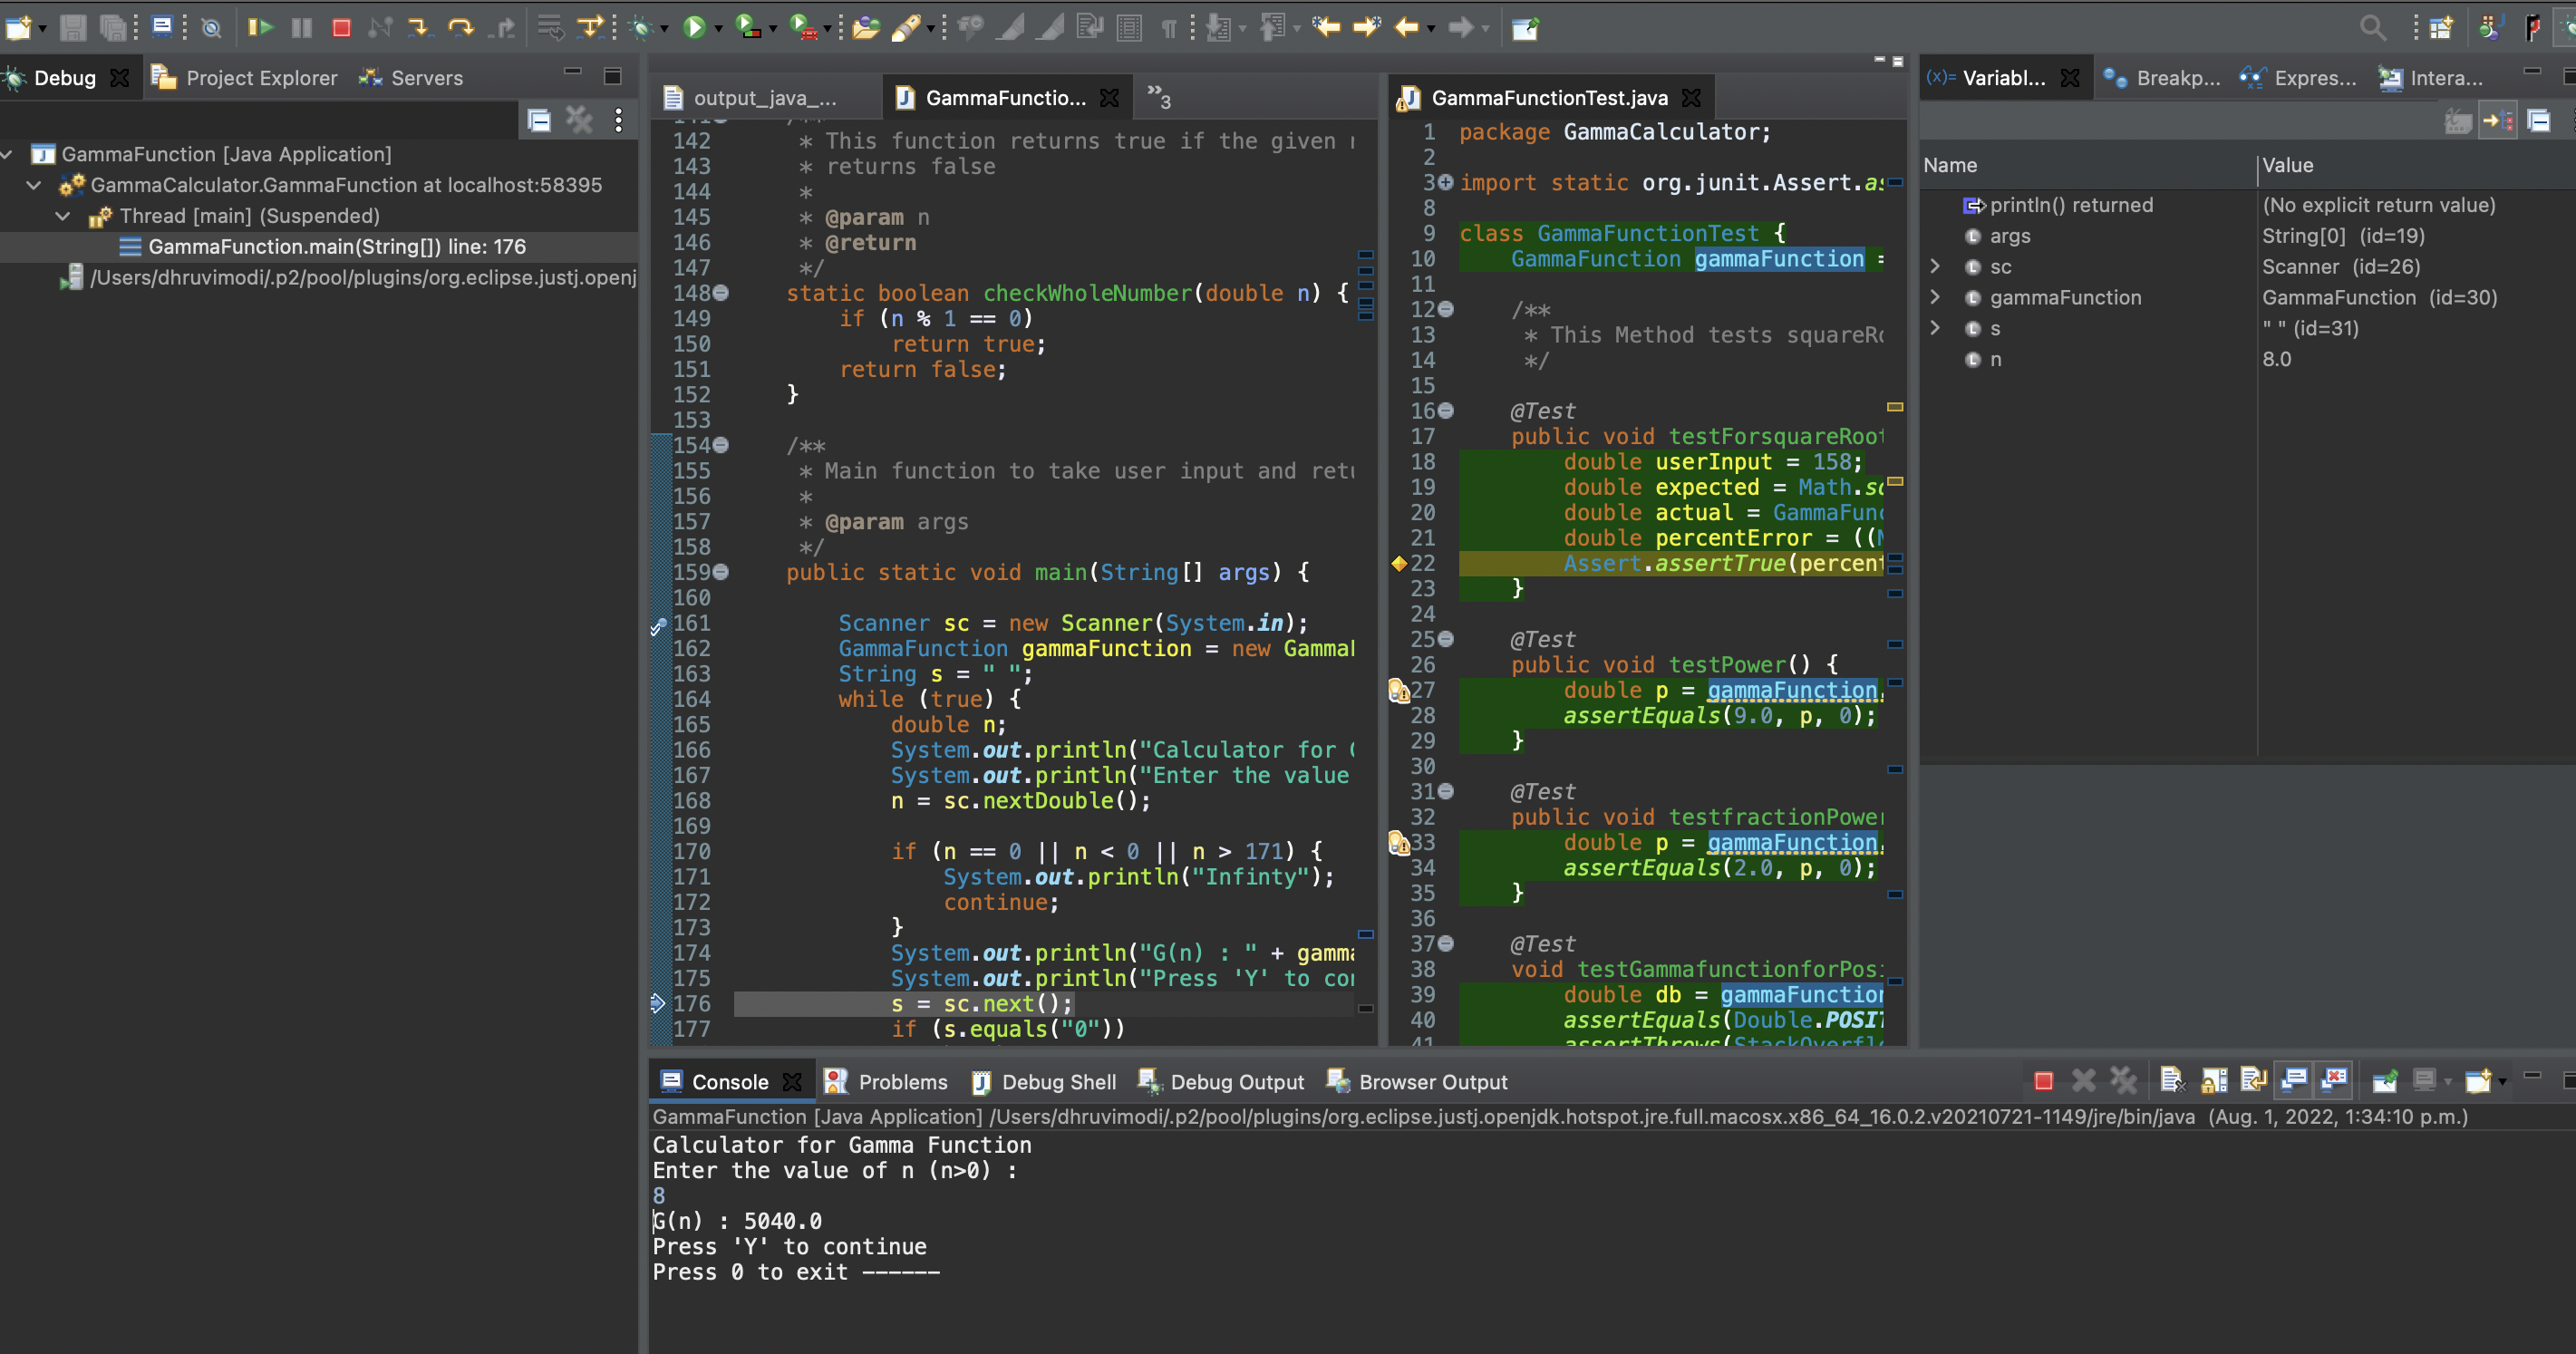
\includegraphics[width=0.9\linewidth]{Images/Debugger.jpg}
    \caption{Screenshot of debugging of Gamma Function.}
    \label{fig:Debugger}
\end{figure}

\section{Tool-Checkstyle}
Java developers can use the Open Source development tool Checkstyle to make sure their code complies with a set of coding standards. The static source code analyzer Checkstyle is integrated into the Eclipse IDE by the Eclipse Checkstyle Plugin (eclipse-cs).

\subsection{Advantages}
\begin{itemize}
    \item{Due to the fact that checkstyle was initially intended to be an independent framework, it is much simpler to combine it with other technologies.}
    
    \item{Code specification verification can be automated with CheckStyle, the key components of the checking include Javadoc comments, name conventions, titles, line lengths, the use of imports and scope modifiers, intervals between characters, etc.}
    
    \item{Team projects benefit from improved code readability, higher project quality, and simpler project maintenance.}
    
    \item{It has the expertise its own rules for developers. Although checkstyle includes more styles than Eclipse does and allows programmers to create their own unique rules,}
\end{itemize}

\subsection{Disadvantages}
\begin{itemize}
    \item{Javac must be able to compile the code in order to find legitimate violations. If not, parsing errors are challenging to comprehend.}
    
    \item{It is difficult to ascertain the type of an expression and its whole inheritance structure.}
    
    \item{The binary Byte Order Mark (BOM) of a file cannot be handled effectively by Checkstyle. In addition, each file is processed separately, making it impossible to view the contents of other files while doing checks.}
\end{itemize}

\begin{figure}[h]
    \centering
    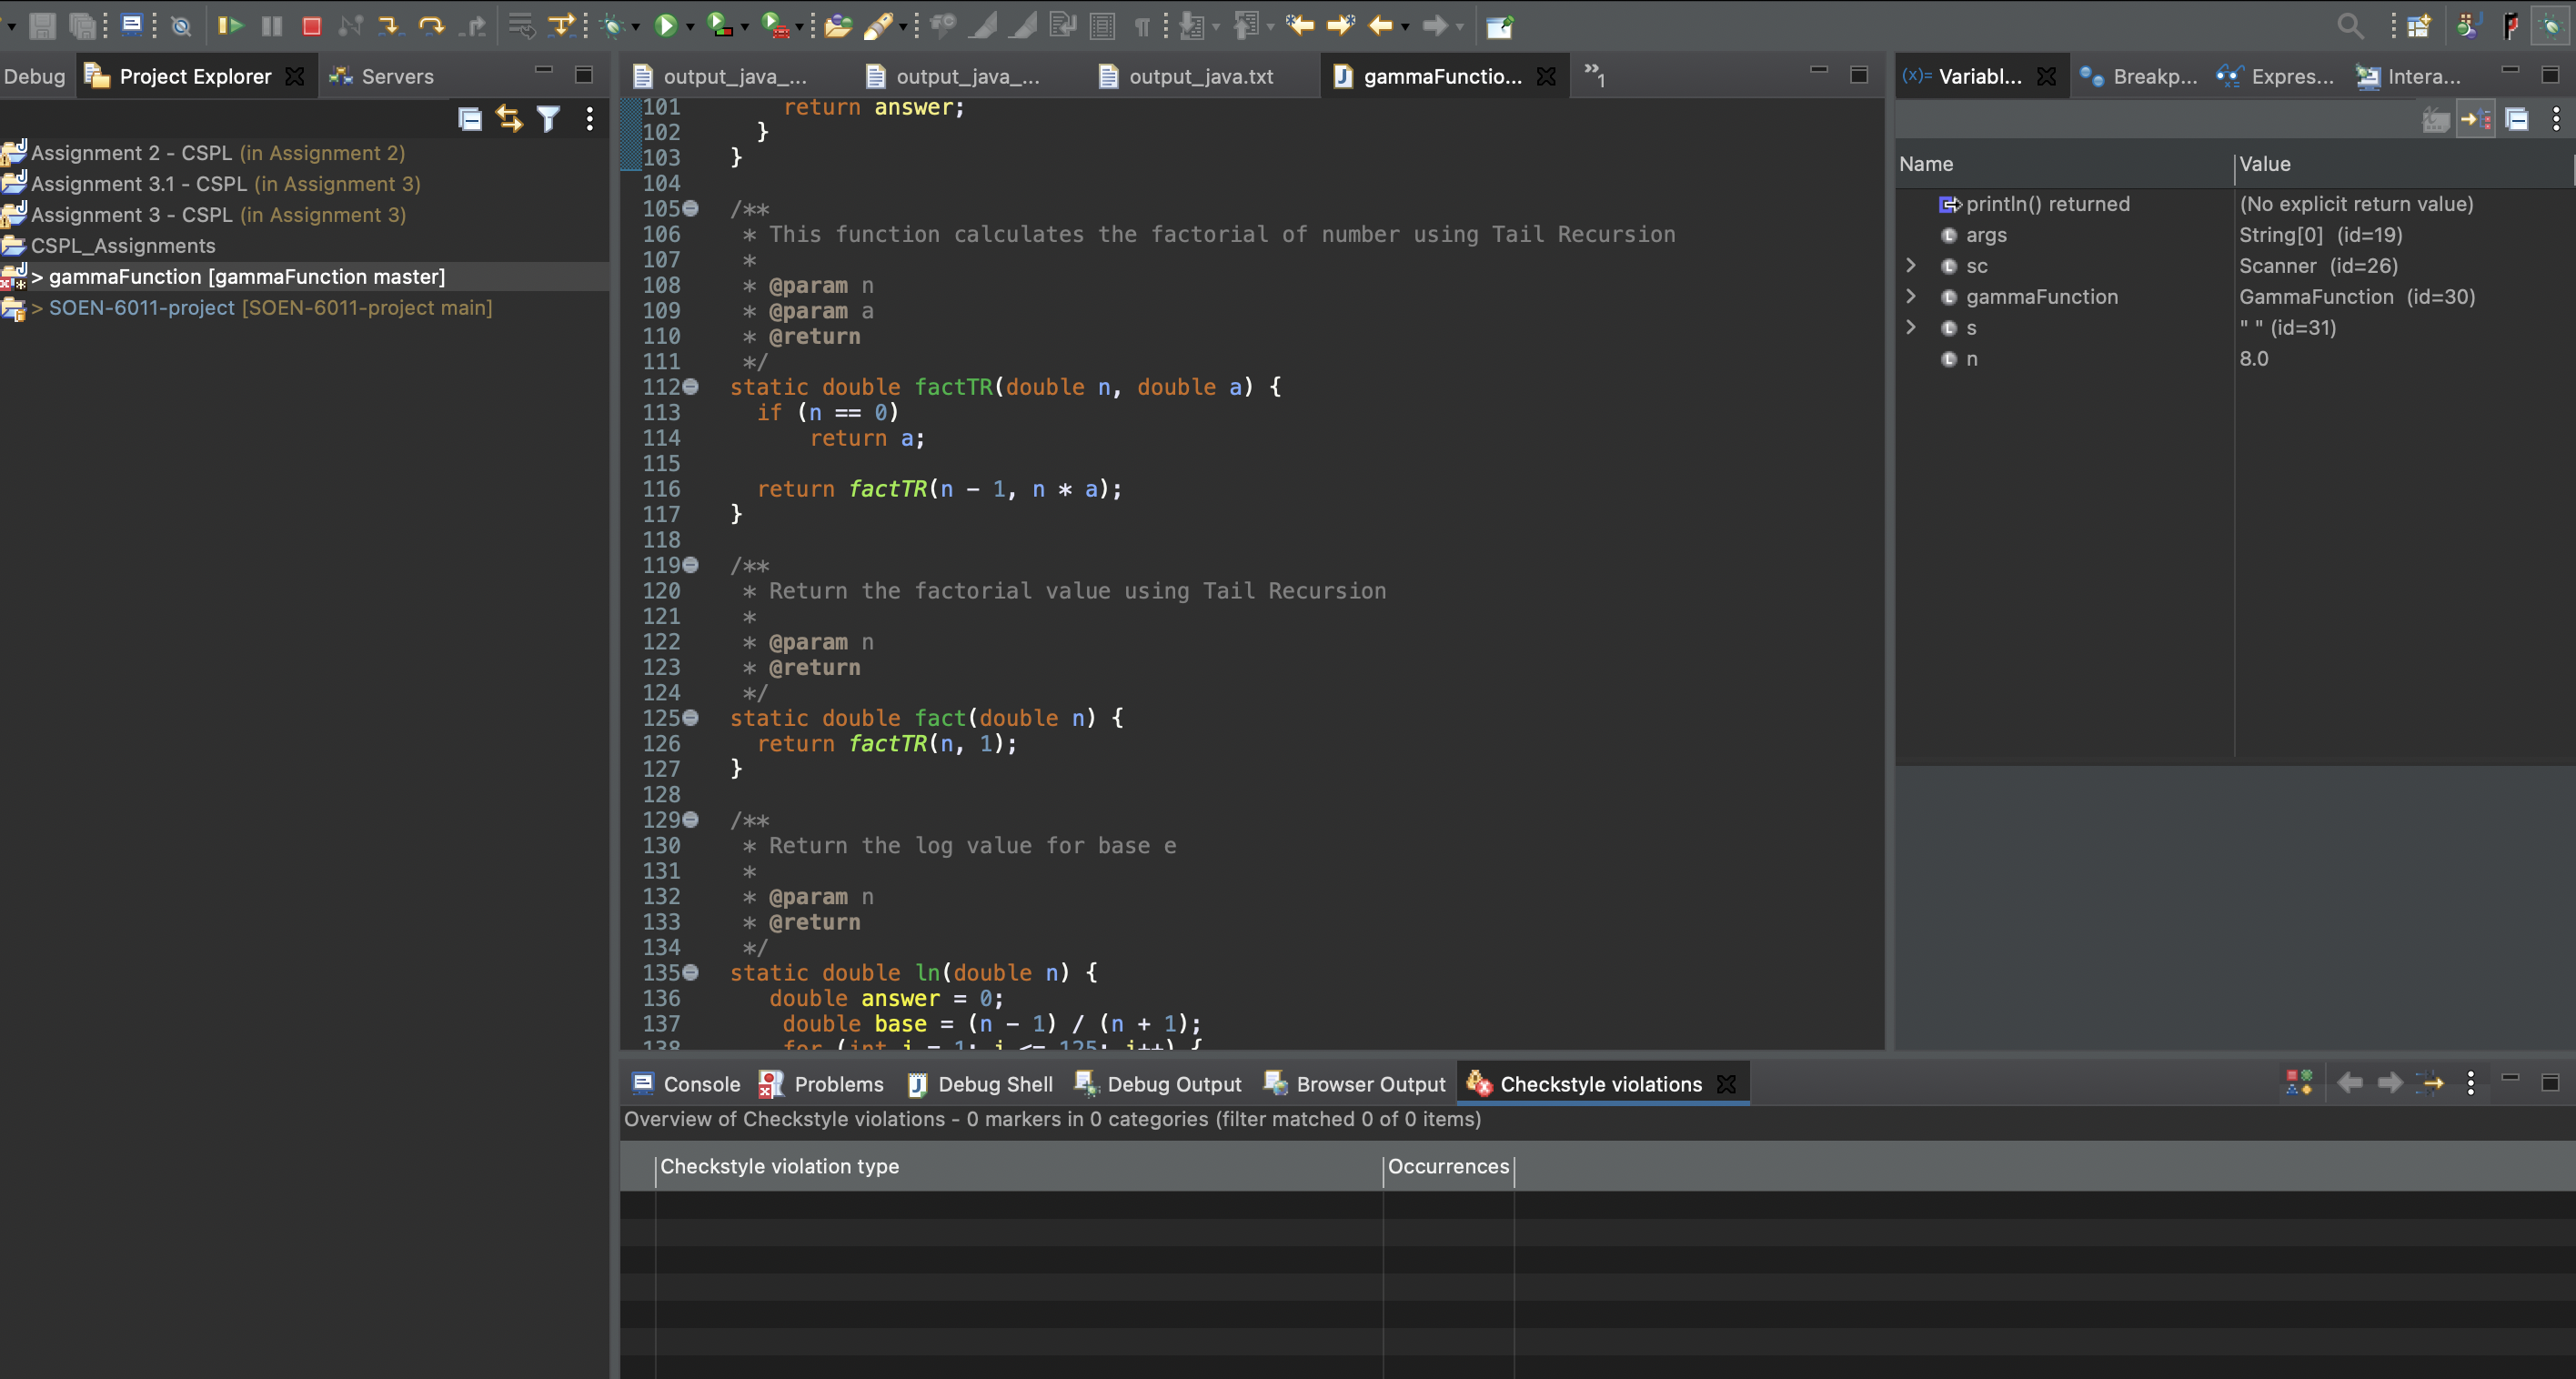
\includegraphics[width=0.9\linewidth]{Images/Typechecking.jpg}
    \caption{Screenshot of Checkstyle of Gamma Function.}
    \label{fig: Checkstyle tool}
\end{figure}

\newpage


\chapter{Problem 5}

\section{Unit test cases}

\subsection{Test Case 1}
\begin{itemize}
    \item \textbf{ID} : TC1
    \item \textbf{Requirement ID} : FR1, FR2, FR4
    \item \textbf{Name of Test Case} : testGammafunctionforPositiveInteger()
    \item \textbf{Test Priority} : High
    \item \textbf{Pre-condition} : Start the programme, then type a value into the console.
    \item \textbf{Test Data} : 142, 234
    \item \textbf{Expected Outcome} : 1.8981437590761713E243, $\infty$
    \item \textbf{Actual Outcome} : 1.8981437590761713E243, $\infty$
    \item \textbf{Test Result} : Success
\end{itemize}

\subsection{Test Case 2}
\begin{itemize}
    \item \textbf{ID} : TC2
    \item \textbf{Requirement ID} : FR2, FR5
    \item \textbf{Name of Test Case} : testGammafunctionforDecimalNumber()
    \item \textbf{Test Priority} : High
    \item \textbf{Pre-condition} : Start the programme, then type a value into the console.
    \item \textbf{Test Data} : 21.14
    \item \textbf{Expected Outcome} : 3.699869886541974E18
    \item \textbf{Actual Outcome} : 3.699869886541974E18
    \item \textbf{Test Result} : Success
\end{itemize}

\subsection{Test Case 3}
\begin{itemize}
    \item \textbf{ID} : TC3
    \item \textbf{Requirement ID} : FR3
    \item \textbf{Name of Test Case} : testGammafunctionforPositiveInteger()
    \item \textbf{Test Priority} : High
    \item \textbf{Pre-condition} : Start the programme, then type a value into the console.
    \item \textbf{Test Data} : 0, -12
    \item \textbf{Expected Outcome} : Exception, Exception
    \item \textbf{Actual Outcome} : Exception, Exception
    \item \textbf{Test Result} : Success
\end{itemize}

\subsection{Test Case 4}
\begin{itemize}
    \item \textbf{ID} : TC4
    \item \textbf{Requirement ID} : FR3
    \item \textbf{Name of Test Case} : testPositiveLimitForGammaFunction()
    \item \textbf{Test Priority} : Medium
    \item \textbf{Pre-condition} : Start the programme, then type a value into the console.
    \item \textbf{Test Data} : 175
    \item \textbf{Expected Outcome} : $+\infty$
    \item \textbf{Actual Outcome} : Exception, Exception
    \item \textbf{Test Result} : Success
\end{itemize}

\subsection{Test Case 5}
\begin{itemize}
    \item \textbf{ID} : TC5
    \item \textbf{Requirement ID} : FR1
    \item \textbf{Name of Test Case} : testMainmethod()
    \item \textbf{Test Priority} : High
    \item \textbf{Pre-condition} : Start the programme, then type a value into the console.
    \item \textbf{Test Data} : 9 y ghjk 0 -4 200 67 y 150 0
    \item \textbf{Expected Outcome} : 40320.0, Exception, Exception, Error message, Error message, $\infty$, 5.443449390774432E92, Exception, 3.8089226376305687E260, Error message
    \item \textbf{Actual Outcome} : 40320.0, Exception, Exception, Error message, Error message, $\infty$, 5.443449390774432E92, Exception, 3.8089226376305687E260, Error message
    \item \textbf{Test Result} : Success
\end{itemize}


\subsection{Conclusion}
The Junit testing with the Junit 5 standard is used to test the Gamma Function programme. The running result and the expected outcome are compared using a series of "assertion" methods to determine whether all test cases either succeed or fail.

\begin{thebibliography}{15}

\addcontentsline{toc}{chapter}{Bibliography}

\indent\indent
Gamma function \\
https://en.wikipedia.org/wiki/Gamma function\\ \\

[Reference Resource] Function \\ https://www.physics.uoguelph.ca/chapter-2-gamma-function\\ \\

\setlength{\parindent}{1em}
29148-2018 --- ISO/IEC/IEEE International Standard -- Systems and software engineering -- Life cycle processes -- Requirements engineering. (2018, November 30). Retrieved from https://standards.ieee.org/standard/29148-2018.html \\ \\

Stirling's Formula.\\
https://mathworld.wolfram.com/StirlingsApproximation.html\\ \\


Stirling's approximation. \\ https://en.wikipedia.org/wiki/Stirling's-approximation-An-alternative-derivation \\ \\


Lanczos approximation.\\ https://en.wikipedia.org/wiki/Lanczos-approximation \\ \\

Exception Handling in JAVA\\
\href{https://www.geeksforgeeks.org/exceptions-in-java/}{https://www.geeksforgeeks.org/exceptions-in-java/} \\ \\

Debugging \\
https://www.techtarget.com/searchsoftwarequality/definition/debugging\\ \\


Google CheckStyle for JAVA Programming\\
https://checkstyle.sourceforge.io/google\_style.html \\ \\


\end{thebibliography}

\end{document}